\subsection{信号的正交变换}

\subsubsection{信号的级数展开}

\begin{definition}[信号的级数展开]
    考虑使用一组函数 $\{\varphi_i(t)\}$,将信号 $x(t) \in L^2(\set{R})$ 展开成级数,即
    \begin{align*}
        x(t) = \sum_{i = -\infty}^{+\infty}c_i\varphi_i(t),
    \end{align*}
    这一形式称为信号 $x(t)$ 的\bd{级数展开}。

    通常,展开系数 $c_i$ 使用信号 $x(t)$ 的某种积分形式来确定。这一积分公式(即求展开系数的公式)
    称之为\bd{信号变换}。
\end{definition}

\subsubsection{函数的正交变换}

\begin{definition}[函数的正交变换]
    若信号级数展开的基函数 $\{\varphi_i(t)\}$ 为标准完备正交函数集,则积分变换
    \begin{align*}
        c_i = \int_{t_1}^{t_2}x(t)\varphi_i^*(t)\D{t}
    \end{align*}
    称为信号 $x(t)$ 的\bd{正交变换},亦称为 \bd{Karhunen-Loève 变换}。
\end{definition}

\begin{note}
    如果信号为符合狄义赫利(Dirichlet)条件的周期函数,则正交分解的系数 $c_i$ 的形式会很漂亮。
\end{note}

\subsubsection{周期函数的正交分解}

\begin{definition}[狄义赫利条件]
    设有一信号 $f(t)$,若它满足以下条件:
    \begin{enumerate}[label=(\arabic*)]
        \item $f(t)$ 间断点的个数有限,
        \item $f(t)$ 极值点的个数有限,
        \item $f(t)$ 绝对积分数值有限,
    \end{enumerate}
    则称 $f(t)$ 满足\bd{狄义赫利条件}。
\end{definition}

\begin{property}
    满足狄义赫利条件的\bd{周期函数}
    都可以在\bd{一组完备的正交基函数}上展开成为\bd{无穷级数}。
\end{property}

\begin{definition}[傅里叶级数展开]
    如果完备的正交函数集是三角函数集或指数函数集,
    则周期函数展成的级数就是\bd{傅里叶级数}。
    相应的级数通常被称为\bd{三角形式傅里叶级数}和{指数形式傅里叶级数}。
\end{definition}

\begin{note}
    回忆三角函数集和指数函数集的定义:
    \begin{itemize}
        \item 三角函数集:$\{1, \cos(\omega_0t + \varphi_1), \cos(2\omega_0t + \varphi_2), \cdots, \cos(n\omega_0 t + \varphi_n)\}$,
            即 $\{1, \cos(n\omega_0t), \sin(n\omega_0t)\}$,其中 $n \in \set{N}^{+}$。
        \item 指数函数集:$\{\mathe^{\mathi n\omega_0t} \mid n \in \set{Z}\}$。
    \end{itemize}
    请注意,三角函数集中的 $n$ 是\bd{正整数},而指数函数集中的 $n$ 是\bd{整数}。
\end{note}

\begin{definition}[三角形式傅里叶级数]
    设周期函数 $f(t)$ 的周期为 $T$,函数集 $\{1, \cos(n\omega_0t), \sin(n\omega_0t)\}$ 是一组完备的正交函数集,其中 $n \in \set{N}^{+}$。
    令 $\omega = 2\pi/T$,则将 $f(t)$ 可以展开成三角函数的无穷级数形式:
    \begin{align*}
        f(t) = a_0 + \sum_{n = 1}^{+\infty}a_n\cos(n\omega t) + b_n\sin(n\omega t),
    \end{align*}
    系数 $a_n$ 和 $b_n$ 统称为\bd{三角形式的傅里叶级数系数},简称为\bd{傅里叶系数}。
\end{definition}

\begin{lemma}
    设周期函数 $f(t)$ 的周期为 $T$,函数集 $\{1, \cos(n\omega_0t), \sin(n\omega_0t)\}$ 是一组完备的正交函数集,其中 $n \in \set{N}^{+}$。
    令 $\omega = 2\pi/T$,则
    \begin{align*}
        \int_{t_0}^{t_0 + T}\cos(m\omega t)\cos (n\omega t)\D{t} & = \begin{cases}
            T / 2, & m = n \neq 0, \\
            T, & m = n = 0, \\
            0, & m \neq n.
        \end{cases} \\
        \int_{t_0}^{t_0 + T}\sin(m\omega t)\sin (n\omega t)\D{t} & = \begin{cases}
            T / 2, & m = n \neq 0, \\
            0, & \text{otherwise}.
        \end{cases} \\
        \int_{t_0}^{t_0 + T}\cos(m\omega t)\sin (n\omega t)\D{t} & = 0.
    \end{align*}
\end{lemma}

\begin{proof}
    首先证明 $\cos(m\omega t)\cos(n\omega t)$ 的积分:
    \begin{align*}
        \int_{t_0}^{t_0 + T}\cos(m\omega t)\cos(n\omega t)\D{t}
        & = \frac{1}{2}\int_{t_0}^{t_0 + T}\left(\cos((m + n)\omega t) + \cos((m - n)\omega t)\right)\D{t} \\
        & = \begin{cases}
            T / 2, & m = n \neq 0, \\
            T, & m = n = 0, \\
            0, & m \neq n.
        \end{cases}
    \end{align*}
    然后证明 $\sin(m\omega t)\sin(n\omega t)$ 的积分:
    \begin{align*}
        \int_{t_0}^{t_0 + T}\sin(m\omega t)\sin(n\omega t)\D{t}
        & = \frac{1}{2}\int_{t_0}^{t_0 + T}\left(\cos((m - n)\omega t) - \cos((m + n)\omega t)\right)\D{t} \\
        & = \begin{cases}
            T / 2, & m = n \neq 0, \\
            0, & \text{otherwise}.
        \end{cases}
    \end{align*}
    最后证明 $\cos(m\omega t)\sin(n\omega t)$ 的积分:
    \begin{align*}
        \int_{t_0}^{t_0 + T}\cos(m\omega t)\sin(n\omega t)\D{t}
        & = \frac{1}{2}\int_{t_0}^{t_0 + T}\left(\sin((m + n)\omega t) - \sin((m - n)\omega t)\right)\D{t} \\
        & = 0.
    \end{align*}
    命题得证。
\end{proof}

\begin{corollary}
    傅里叶系数 $a_n$ 和 $b_n$ 的表达式为:
    \begin{align*}
        a_0 & = \frac{1}{T}\int_{t_0}^{t_0 + T}f(t)\D{t}, \\
        a_n & = \frac{2}{T}\int_{t_0}^{t_0 + T}f(t)\cos(n\omega t)\D{t}, \\
        b_n & = \frac{2}{T}\int_{t_0}^{t_0 + T}f(t)\sin(n\omega t)\D{t}.
    \end{align*}
\end{corollary}

\begin{proof}
    已知 $f(t) = a_0 + \sum_{n = 1}^{+\infty}a_n\cos(n\omega t) + b_n\sin(n\omega t)$,则
    等式两边同时在 $[t_0, t_0 + T]$ 上积分,有
    \begin{align*}
        \int_{t_0}^{t_0 + T}f(t)\D{t} & = \int_{t_0}^{t_0 + T}a_0\D{t} + \sum_{n = 1}^{+\infty}\int_{t_0}^{t_0 + T}a_n\cos(n\omega t)\D{t} + \sum_{n = 1}^{+\infty}\int_{t_0}^{t_0 + T}b_n\sin(n\omega t)\D{t} \\
        & = \int_{t_0}^{t_0 + T}a_0\D{t} + \sum_{n = 1}^{+\infty}a_n\int_{t_0}^{t_0 + T}\cos(n\omega t)\D{t} + \sum_{n = 1}^{+\infty}b_n\int_{t_0}^{t_0 + T}\sin(n\omega t)\D{t} \\
        & = T \cdot a_0 + \sum_{n = 1}^{+\infty}a_n\cdot 0 + \sum_{n = 1}^{+\infty}b_n\cdot 0 \\
        & = T \cdot a_0.
    \end{align*}
    因此,有 $a_0 = \frac{1}{T}\int_{t_0}^{t_0 + T}f(t)\D{t}$。

    同理,在等式左右两侧乘上 $\cos(n \omega t)$ 之后再在 $[t_0, t_0 + T]$ 上积分,
    可得 $a_n = \frac{2}{T}\int_{t_0}^{t_0 + T}f(t)\cos(n\omega t)\D{t}$。
    在等式左右两侧乘上 $\sin(n \omega t)$ 之后再在 $[t_0, t_0 + T]$ 上积分,
    可得可得 $b_n = \frac{2}{T}\int_{t_0}^{t_0 + T}f(t)\sin(n\omega t)\D{t}$。
    命题得证。
\end{proof}

\begin{remark}
    常用的正交函数集的基本函数,除正弦型函数(含复指数函数)外,
    还有勒让德函数(Legendre function)、贝塞尔函数(Bessel function)、
    沃尔什函数(Walsh function)等,不一一列举。
\end{remark}

\begin{definition}[复指数形式傅里叶级数]
    由欧拉公式可以得到 $\cos(n\omega t) = (\mathe^{\mathi n\omega t} + \mathe^{-\mathi n\omega t}) / 2$,
    以及 $\sin(n\omega t) = (\mathe^{\mathi n\omega t} - \mathe^{-\mathi n\omega t}) / 2\mathi$。
    因此,我们可以将三角函数形式的傅里叶级数改写为:
    \begin{align*}
        f(t) = a_0 + \sum_{i = 1}^{+\infty}\left(\frac{a_n - \mathi b_n}{2}\mathe^{\mathi n\omega t} + \frac{a_n + \mathi b_n}{2}\mathe^{-\mathi n\omega t}\right).
    \end{align*}
    记 $F(\cdot)$ 为一个函数,则 $a_0, a_n, b_n$ 可以看做是 $(n, \omega)$ 对应的函数值。则
    \begin{align*}
        f(t) = F(0) + \sum_{i = 1}^{+\infty}\left(F(n\omega)+ F(-n\omega)\right)
    \end{align*}
    再记 $F_n = F(n\omega)$,则可将 $f(t)$ 表示为\bd{复指数形式的傅里叶级数}:
    \begin{align*}
        f(t) = \sum_{n = -\infty}^{+\infty}F_n\mathe^{\mathi n\omega t},
    \end{align*}
    其中 $F_n = (a_n - \mathi b_n) / 2$ 为\bd{复指数形式的傅里叶级数系数}。
\end{definition}

\begin{property}
    复指数形式傅里叶级数的系数 $F_n$ 的表达式为:
    \begin{align*}
        F_n = \frac{1}{T}\int_{t_0}^{t_0 + T}f(t)\mathe^{-\mathi n\omega t}\D{t}.
    \end{align*}
\end{property}

\begin{proof}
    (方法一)
    \begin{align*}
        F_n & = \frac{a_n - \mathi b_n}{2} \\
        & = \frac{1}{2} \cdot \frac{2}{T}\int_{t_0}^{t_0 + T}f(t)\cos(n\omega t)\D{t} - \frac{\mathi}{2} \cdot \frac{2}{T}\int_{t_0}^{t_0 + T}f(t)\sin(n\omega t)\D{t} \\
        & = \frac{1}{T}\int_{t_0}^{t_0 + T}f(t)(\cos(n\omega t) - \mathi \sin(n\omega t))\D{t} \\
        & = \frac{1}{T}\int_{t_0}^{t_0 + T}f(t)\mathe^{-\mathi n\omega t}\D{t}.
    \end{align*}
    命题得证。
\end{proof}

\begin{proof}
    (方法二)
    由级数展开的定义,在函数集 $\{\mathe^{\mathi n\omega t}\}$ 上展开,有
    \begin{align*}
        F_n & = \frac{\ip{f}{\varphi_n}}{\ip{\varphi_n}{\varphi_n}}\\
        & = \frac{1}{k_n}\int_{t_0}^{t_0 + T}f(t) \mathe^{-\mathi n\omega t}\D{t}.
    \end{align*}
    而 $k_n$ 可以计算如下:
    \begin{align*}
        k_n & = \int_{t_0}^{t_0 + T}\mathe^{\mathi n\omega t}\mathe^{-\mathi n\omega t}\D{t} \\
        & = \int_{t_0}^{t_0 + T}\D{t} \\
        & = T.
    \end{align*}
    因此 $F_n = \frac{1}{T}\int_{t_0}^{t_0 + T}f(t)\mathe^{-\mathi n\omega t}\D{t}$。
\end{proof}

\begin{property}
    对偶信号序列的傅里叶级数而言,$F_n$ 是偶对称的实数序列,
    对奇信号序列的傅里叶级数而言,$F_n$ 是奇对称的纯虚序列。
\end{property}

\begin{proof}
    考虑关系式 $F_n = (a_n - \mathi b_n) / 2$:
    \begin{itemize}
        \item 对于偶信号序列而言,$a_n \neq 0, b_n = 0$,所以 $F_n$ 只有直流分量和余弦项。
        \item 对于奇信号序列而言,$a_n = 0, b_n \neq 0$,所以 $F_n$ 只有正弦项。
    \end{itemize}
    命题得证。
\end{proof}

\begin{corollary}[帕斯瓦尔定理的推论]
    周期信号的\bd{平均功率}等于傅里叶级数展开各谐波分量有效值的平方和。
    也就是说,\bd{时域和频域的能量守恒}。
\end{corollary}

\begin{proof}
    由帕斯瓦尔定理知,
    \begin{align*}
        \int_{t_0}^{t_0 + T}\|f(t)\|^2\D{t} & = \|a_0\|^2\cdot k_0
            + \sum_{i = 1}^{+\infty}\|a_i\|^2k_{\cos, i}
            + \sum_{i = 1}^{+\infty}\|b_i\|^2k_{\sin, i} \\
        & = T \cdot \|a_0\|^2 + \frac{T}{2}\cdot \sum_{i = 1}^{+\infty}(\|a_i\|^2 + \|b_i\|^2).
    \end{align*}
    因此,有
    \begin{align*}
        P & = \overline{\|f(t)\|^2} = \frac{1}{T}\int_{t_0}^{t_0 + T}\|f(t)\|^2\D{t} \\
        & = \frac{1}{T}\left(T \cdot \|a_0\|^2 + \frac{T}{2}\cdot \sum_{i = 1}^{+\infty}(\|a_i\|^2 + \|b_i\|^2)\right) \\
        & = \|a_0\|^2 + \frac{1}{2}\sum_{i = 1}^{+\infty}(\|a_i\|^2 + \|b_i\|^2) \\
        & = \sum_{i = -\infty}^{+\infty}\|F_n\|^2.
    \end{align*}
    命题得证。
\end{proof}

\subsubsection{周期信号的傅里叶级数}

\begin{definition}
    
    % TODO: 没看懂 PPT

    周期信号的傅里叶级数可视化如图 \ref{fig:periodic-signal-fourier-series} 所示。
    \begin{figure}[H]
        \centering
        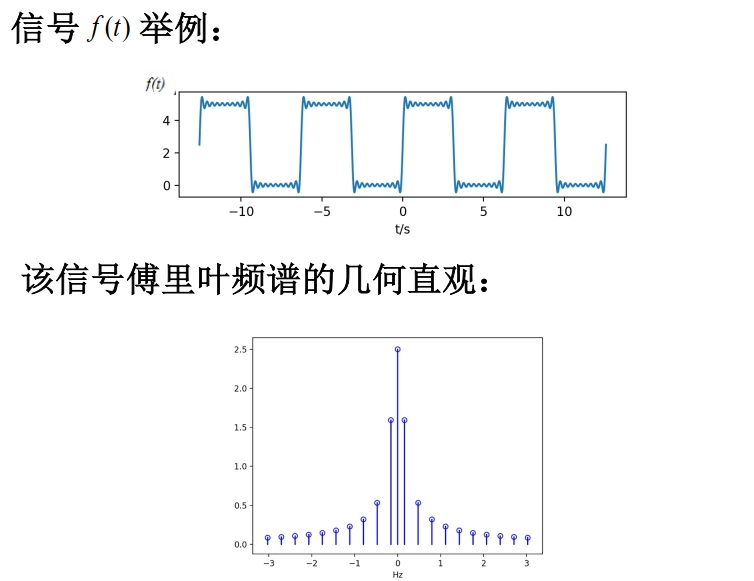
\includegraphics[width = 0.6\textwidth]{chap2/img/periodic-signal-fourier-series.png}
        \caption{周期信号的傅里叶级数}
        \label{fig:periodic-signal-fourier-series}
    \end{figure}
\end{definition}

\begin{property}[周期信号的傅里叶频谱特点]
    周期信号的傅里叶频谱有以下特点:
    \begin{itemize}
        \item 仅在一些离散的频率点 $n\omega$ 上有值。
        \item 离散间隔为 $\omega = 2\pi f = 2\pi / T$。
        \item $F_n$ 是双边谱,即 $F_n = F_{-n}$,因此正负频率的频谱幅度相加才是实际幅度。
        \item 信号的功率为 $\sum_{-\infty}^{+\infty}\|F_n\|^2$。
    \end{itemize}
\end{property}

\begin{example}[周期矩形脉冲信号的傅里叶级数]
    设周期矩形脉冲信号 $f(t)$ 的脉冲宽度为 $\tau$,脉冲幅度为 $E$,重复周期为 $T$。
    图像如图 \ref{fig:periodic-rect-pulse-signal} 所示。
    \begin{figure}[H]
        \centering
        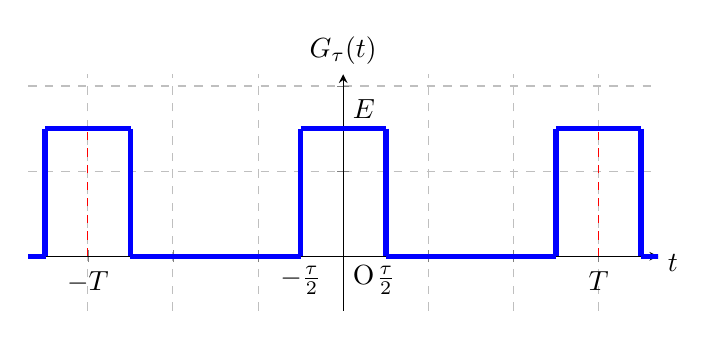
\begin{tikzpicture}
            \begin{axis}[
                axis lines = middle,
                xlabel = {$t$},
                xlabel style={at={(rel axis cs:1, 0.2)}, anchor=west},
                ylabel = {$G_{\tau}(t)$},
                ylabel style={at={(rel axis cs:0.5, 1)}, anchor=south},
                xmin = -3.7, xmax = 3.7,
                ymin = -0.2, ymax = 1.7,
                grid = major,
                grid style = dashed,
                scale only axis,
                width = 8cm,
                height = 3cm,
                axis equal,
                xtick = {-3, -2, -1, 0, 1, 2, 3},
                xticklabels = {$-T$, $ $, $ $, $ $, $ $, $ $, $T$},
                ytick = {0, 1, 2},
                yticklabels = {$ $, $ $, $ $},
            ]
            \addplot[domain=-3.7:-3.5, samples=100, smooth, line width=2pt, blue] {0};
            \addplot[smooth, line width=2pt, blue] coordinates {(-3.5, 0) (-3.5, 1.5)};
            \addplot[dashed, red] coordinates {(-3, 0) (-3, 1.5)};
            \addplot[domain=-3.5:-2.5, samples=100, smooth, line width=2pt, blue] {1.5};
            \addplot[smooth, line width=2pt, blue] coordinates {(-2.5, 1.5) (-2.5, 0)};
            \addplot[domain=-2.5:-0.5, samples=100, smooth, line width=2pt, blue] {0};
            \addplot[smooth, line width=2pt, blue] coordinates {(-0.5, 0) (-0.5, 1.5)};
            \addplot[domain=-0.5:0.5, samples=100, smooth, line width=2pt, blue] {1.5};
            \addplot[smooth, line width=2pt, blue] coordinates {(0.5, 1.5) (0.5, 0)};
            \addplot[domain=0.5:2.5, samples=100, smooth, line width=2pt, blue] {0};
            \addplot[smooth, line width=2pt, blue] coordinates {(2.5, 0) (2.5, 1.5)};
            \addplot[domain=2.5:3.5, samples=100, smooth, line width=2pt, blue] {1.5};
            \addplot[dashed, red] coordinates {(3, 0) (3, 1.5)};
            \addplot[smooth, line width=2pt, blue] coordinates {(3.5, 1.5) (3.5, 0)};
            \addplot[domain=3.5:3.7, samples=100, smooth, line width=2pt, blue] {0};
            \node at (axis cs:0, 0) [anchor=north west] {O};
            \node at (axis cs:0, 1.5) [anchor=south west] {$E$};
            \node at (axis cs:-0.5, 0) [anchor = north] {$-\frac{\tau}{2}$};
            \node at (axis cs:0.5, 0) [anchor = north] {$\frac{\tau}{2}$};
            \end{axis}
        \end{tikzpicture}
        \caption{周期矩形脉冲信号}
        \label{fig:periodic-rect-pulse-signal}
    \end{figure}

    则其在频域上的图像如图 \ref{fig:periodic-rect-pulse-signal-freq} 所示。
    \begin{figure}[H]
        \centering
        \begin{tikzpicture}
            \begin{axis}[
                axis lines = middle,
                xlabel = {$\omega$},
                ylabel = {$F_n$},
                ylabel style={at={(rel axis cs:0.5, 1)}, anchor=south},
                xmin = -10, xmax = 10,
                ymin = -0.3, ymax = 1.1,
                xtick = {-10, -8, -6, -4, -2, 0, 2, 4, 6, 8, 10},
                xticklabels = {$ $, $ $, $ $, $ $, $ $, $ $, $ $, $ $, $ $, $ $, $ $},
                ytick distance = 0.25,
                ytick = {-0.25, 0, 0.25, 0.5, 0.75, 1},
                yticklabels = {$ $, $ $, $ $, $ $, $ $, $\dfrac{E\tau}{T}$},
                grid = major,
                grid style = dashed,
            ]
            \addplot[dashed, domain=-10:10, samples=100, smooth, line width=2pt, blue] {sin(deg(x))/x};
            \draw[-stealth, smooth, red] (axis cs:-16.7552, 0) -- (axis cs:-16.7552, -0.0517);
            \draw[-stealth, smooth, red] (axis cs:-12.5664, 0) -- (axis cs:-12.5664, 0);
            \draw[-stealth, smooth, red] (axis cs:-8.3776, 0) -- (axis cs:-8.3776, 0.1034);
            \draw[-stealth, smooth, red] (axis cs:-4.1888, 0) -- (axis cs:-4.1888, -0.2067);
            \draw[-stealth, smooth, red] (axis cs:0, 0) -- (axis cs:0, 1);
            \draw[-stealth, smooth, red] (axis cs:4.1888, 0) -- (axis cs:4.1888, -0.2067);
            \draw[-stealth, smooth, red] (axis cs:8.3776, 0) -- (axis cs:8.3776, 0.1034);
            \draw[-stealth, smooth, red] (axis cs:12.5664, 0) -- (axis cs:12.5664, 0);
            \draw[-stealth, smooth, red] (axis cs:16.7552, 0) -- (axis cs:16.7552, -0.0517);
            
            \node at (axis cs:0, 0) [anchor=north west] {O};
            \node at (axis cs:3.1416, 0) [anchor=north] {$\dfrac{2\pi}{\tau}$};
            \node at (axis cs:6.2832, 0) [anchor=north] {$\dfrac{4\pi}{\tau}$};
            \end{axis}
        \end{tikzpicture}
        \caption{周期矩形脉冲信号的频谱}
        \label{fig:periodic-rect-pulse-signal-freq}
    \end{figure}

    \begin{itemize}
        \item 谱线包络线为 $\sa$ 函数。
        \item 频谱谱线的间隔为 $\omega = 2\pi / T$。
        \item 谱线包络线过零点位置为 $\omega_k = 2k\pi / \tau$,其中 $k \neq 0, k \in \set{Z}$。
        % TODO: 没看懂 PPT
    \end{itemize}
\end{example}

\begin{theorem}
    周期为 $T$,脉冲宽度为 $\tau$,脉冲幅度为 $E$ 的周期矩形脉冲信号,谱线包络线则为
    \begin{align*}
        \frac{E\tau}{T}\sa{\left(\frac{\omega\tau}{2}\right)}.
    \end{align*}
\end{theorem}

\begin{proof}
    \begin{align*}
        F_n & = \frac{1}{T}\int_{-\tau/2}^{\tau/2}E\cdot \mathe^{-\mathi n\omega t}\D{t} \\
        & = \frac{E}{T}\int_{-\tau/2}^{\tau/2}\mathe^{-\mathi n\omega t}\D{t} \\
        & = \frac{E}{T}\cdot\frac{1}{-\mathi n\omega}\cdot\left(\mathe^{-\mathi n\omega t}\right)\Big|_{-\tau/2}^{\tau/2} \\
        & = \frac{E}{T}\cdot\frac{1}{-\mathi n\omega}\cdot\left(\mathe^{-\mathi n\omega \tau / 2} - \mathe^{\mathi n \omega \tau /2 }\right) \\
        & = \frac{E}{T}\cdot\frac{1}{-\mathi n\omega}\cdot\left(-2\mathi\sin\left(\frac{n\omega\tau}{2}\right)\right) \\
        & = \frac{E\tau}{T}\frac{\sin(n\omega\tau/2)}{n\omega\tau/2} \\
        & = \frac{E\tau}{T}\sa{\left(\frac{n\omega\tau}{2}\right)}.
    \end{align*}
\end{proof}

\begin{remark}
    非周期信号,在频率域上则为连续频谱;周期信号,在频率域上则为离散频谱。
    它们之间的转换关系,可以由下图 \ref{fig:periodic-nonperiodic-signal} 描述。
    \begin{figure}[H]
        \centering
        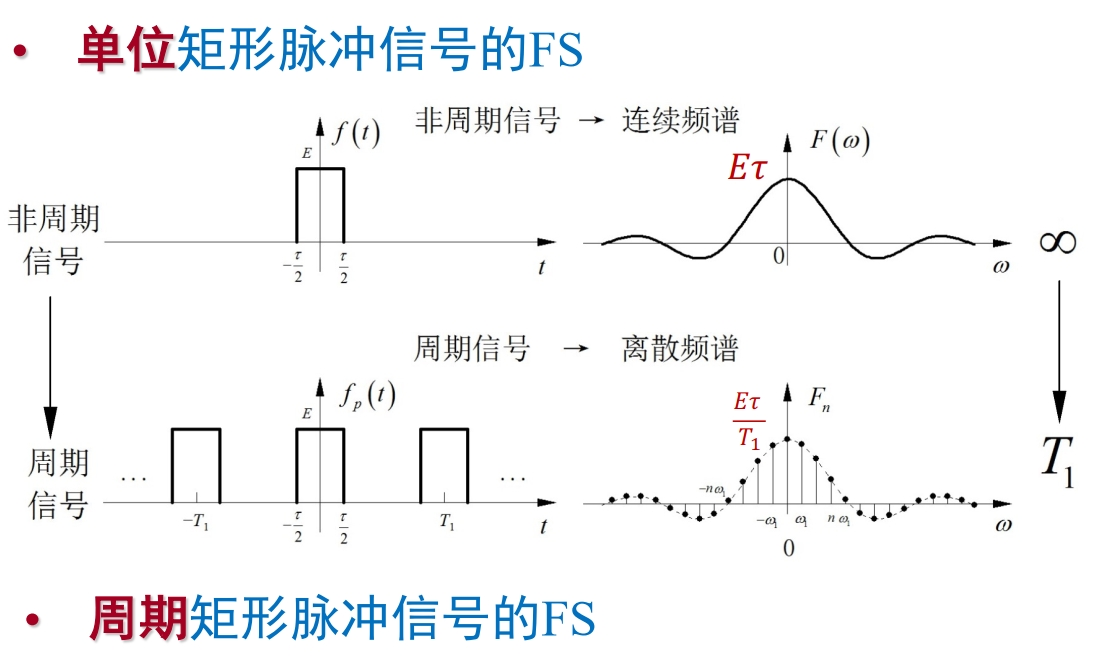
\includegraphics[width = 0.8\textwidth]{chap2/img/periodic-nonperiodic-signal.png}
        \caption{周期信号与非周期信号的频谱}
        \label{fig:periodic-nonperiodic-signal}
    \end{figure}
\end{remark}

\begin{property}[周期矩形脉冲信号的特点]
    在频域,能量主要集中在第一个零点以内!

    实际上,在允许一定失真的条件下,可以要求一个通信系统
    只把 $|\omega| \le 2\pi/\tau$ 频率范围内的各个频率分量传送过去,
    而舍弃 $|\omega| \ge 2\pi/\tau$ 的分量。

    常把 $-2\pi/\tau \le \omega \le 2\pi/\tau$ 这段频率范围成为矩形信号的\bd{频带宽度},
    简称\bd{带宽}。
    带宽只和脉冲的脉宽有关,而与脉高和周期均无关。
\end{property}

\begin{property}[周期信号的频谱谱线的特点]
    周期信号的频谱谱线的\bd{间隔}为
    \begin{align*}
        \omega = \frac{2\pi}{T}.
    \end{align*}

    % TODO: 没看懂 PPT
    
    周期信号的频谱谱线的\bd{长度}为
    \begin{align*}
        F_n = F(n\omega) = \frac{1}{T}\int_{t_0}^{t_0 + T}f(t)\mathe^{-\mathi n\omega t}\D{t}.
    \end{align*}
\end{property}

\begin{note}
    由于复指数完备正交函数集中含有\bd{正负项},故为\bd{双边谱}。
    对于 $n\omega$ 这一频率的频谱而言,频谱幅度为
    \begin{align*}
        |F_n| + |F_{-n}| = 2|F_n| = \frac{1}{2}\left(a_n^2 + b_n^2\right).
    \end{align*}
    一定要注意,它并不是 $|F_n|$。
\end{note}

\begin{exercise}
    已知 $f(t) = \sin t\cos 2t + 5\cos 3t \sin 4t$,求该函数的傅里叶级数。
\end{exercise}

\begin{solution}
    由三角函数的和差化积公式,有
    \begin{align*}
        f(t) & = \frac{1}{2}\left(\sin 3t - \sin t\right) + \frac{5}{2}\left(\sin 7t + \sin t\right) \\
        & = 2\sin t + \frac{1}{2}\sin 3t + \frac{5}{2}\sin 7t.
    \end{align*}
    此即为该函数的傅里叶级数。
\end{solution}

\subsubsection{非周期信号的傅里叶级数}

我们已经掌握了周期信号的傅里叶展开,那么如何处理非周期信号的傅里叶展开呢?
非周期信号可以看成是\bd{周期 $T$ 趋于无限大的周期信号},因此我们可以将非周期信号的傅里叶展开看成是周期信号的极限情况。

\begin{property}[非周期信号频谱性质]
    非周期信号的谱线间隔趋于 $0$,变成了\bd{连续频谱},谱线长度趋于 $0$。
\end{property}

\begin{proof}
    当 $T \to +\infty$ 时,$\omega = 2\pi / T \to 0$,谱线间距变密直至为 $0$。$\omega$ 变为连续域。
    此时
    $F_n = \frac{1}{T}\int_{T}f(t)\mathe^{-\mathi n\omega t} \D{t} \to 0$,谱线高度变矮直至为 $0$。
\end{proof}

\begin{remark}
    从物理意义着手:既然是信号,那么它必定会有能量;无论怎样,能量一定是守恒的。
    因此,频率域一定会以某种形式存在。

    从数学角度思考:无限多无穷小量的和,在极限意义下,可能等于一个有限值。
    谱线高度变矮直至为 $0$,只是说每个分量变成了无穷小量,但没有说总和(信号)为 $0$。
\end{remark}
